\documentclass{article}

\usepackage{graphicx,amsmath}
\usepackage{epstopdf}

\title{Problem3 Report}
\author{Qi Liu}
\date{\today}

\begin{document}

\maketitle

\section{Ideal Lowpass Filter}
The ideal lowpass filter is defined as $$H(u,v)=\begin{cases} 1 & D(u,v)\le D_0 \\ 0 & D(u,v)>D_0 \end{cases}$$ here $D_0$ is radius and $D(u,v)=\sqrt{(u-P/2)^2+(v-Q/2)^2)}$ is the distance from $(u,v)$ to the center.


\includegraphics[width=0.33\textwidth]{../data/characters_test_pattern.jpg}

\includegraphics[width=0.33\textwidth]{../data/ideal_lowpass_10_characters_test_pattern.jpg}

\includegraphics[width=0.33\textwidth]{../data/ideal_lowpass_30_characters_test_pattern.jpg}

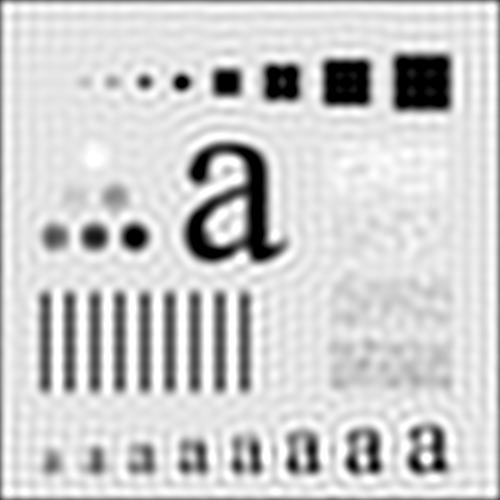
\includegraphics[width=0.33\textwidth]{../data/ideal_lowpass_60_characters_test_pattern.jpg}
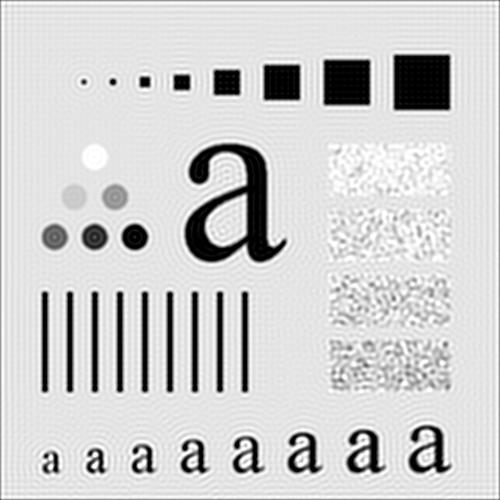
\includegraphics[width=0.33\textwidth]{../data/ideal_lowpass_160_characters_test_pattern.jpg}
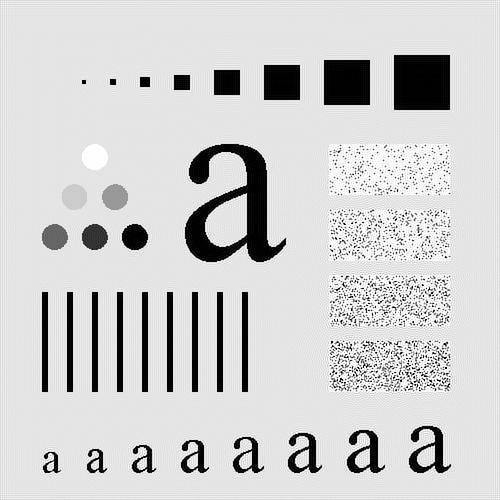
\includegraphics[width=0.33\textwidth]{../data/ideal_lowpass_460_characters_test_pattern.jpg}

The above figures are results of ideal lowpass filter. The first one is the original figure. The second to the sixth figure has different value of $D_0$, which is set by 10, 30, 60, 160 and 460.

\section{Butterworth Lowpass Filter}
The Butterworth lowpass filter is defined as $$H(u,v)=\frac{1}{1+[D(u,v)/D_0]^{2n}}$$ here $D(u,v)$ and $D_0$ have the same meaning above.


\includegraphics[width=0.33\textwidth]{../data/characters_test_pattern.jpg}

\includegraphics[width=0.33\textwidth]{../data/butterworth_lowpass_10_characters_test_pattern.jpg}
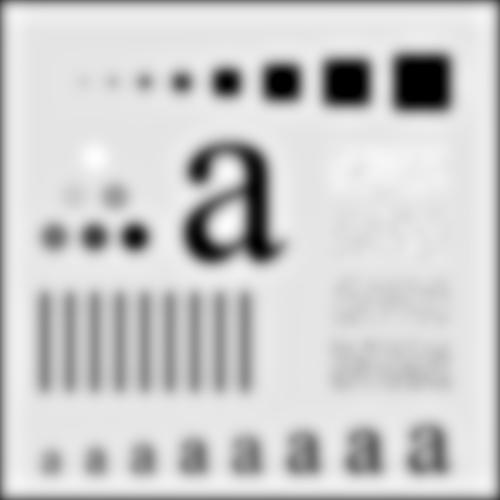
\includegraphics[width=0.33\textwidth]{../data/butterworth_lowpass_30_characters_test_pattern.jpg}

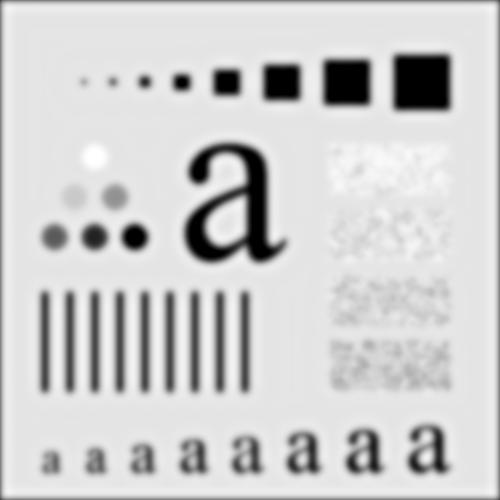
\includegraphics[width=0.33\textwidth]{../data/butterworth_lowpass_60_characters_test_pattern.jpg}

\includegraphics[width=0.33\textwidth]{../data/butterworth_lowpass_160_characters_test_pattern.jpg}

\includegraphics[width=0.33\textwidth]{../data/butterworth_lowpass_460_characters_test_pattern.jpg}

The above figures are results of Butterworth lowpass filter. The first one is the original figure. The second to the sixth figure has different value of $D_0$, which is set by 10, 30, 60, 160 and 460. The value of $n$ is 2.

\section{Gaussian Lowpass Filter}
The Gaussian lowpass filter is defined as $$H(u,v)=\exp({-D^2(u,v)/2D_0^2})$$ here $D(u,v)$ and $D_0$ have the same meaning above.


\includegraphics[width=0.33\textwidth]{../data/characters_test_pattern.jpg}
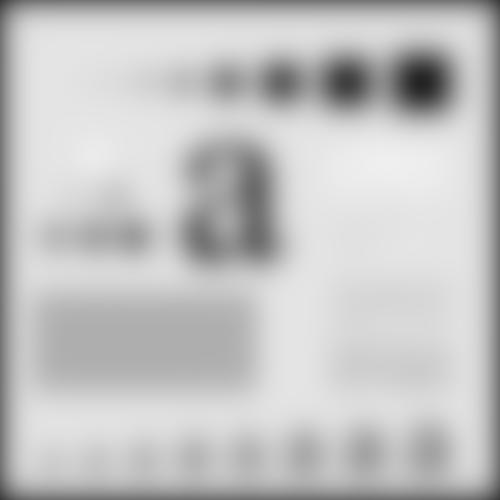
\includegraphics[width=0.33\textwidth]{../data/gaussian_lowpass_10_characters_test_pattern.jpg}
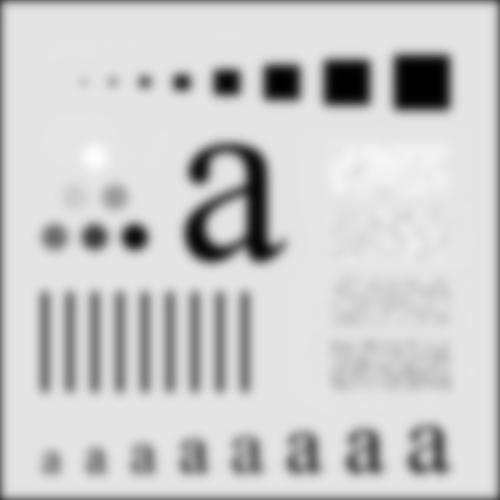
\includegraphics[width=0.33\textwidth]{../data/gaussian_lowpass_30_characters_test_pattern.jpg}

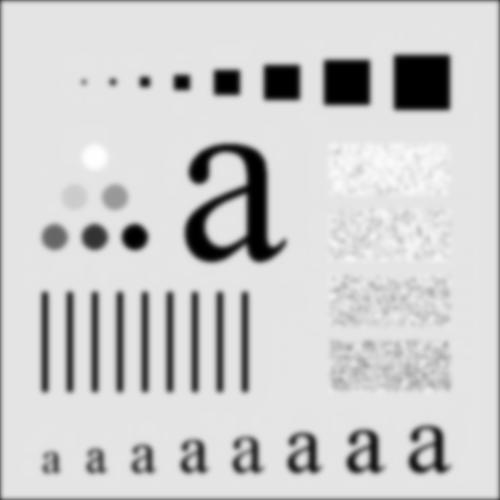
\includegraphics[width=0.33\textwidth]{../data/gaussian_lowpass_60_characters_test_pattern.jpg}

\includegraphics[width=0.33\textwidth]{../data/gaussian_lowpass_160_characters_test_pattern.jpg}

\includegraphics[width=0.33\textwidth]{../data/gaussian_lowpass_460_characters_test_pattern.jpg}

The above figures are results of Gaussian lowpass filter. The first one is the original figure. The second to the sixth figure has different value of $D_0$, which is set by 10, 30, 60, 160 and 460.

\section{Highpass Filter}
The highpass filter can be calculated by one minus the corresponding lowpass filter. The figures below show the result of highpass filter. The first row is ideal highpass filter, the second row is Butterworth highpass filter and the thrid row is Gaussian highpass filter. The figures from left to right have different value of $D_0$ which is 30, 60 and 160.

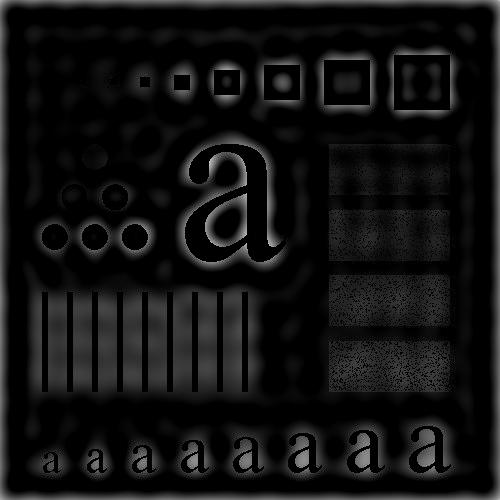
\includegraphics[width=0.33\textwidth]{../data/ideal_highpass_30_characters_test_pattern.jpg}
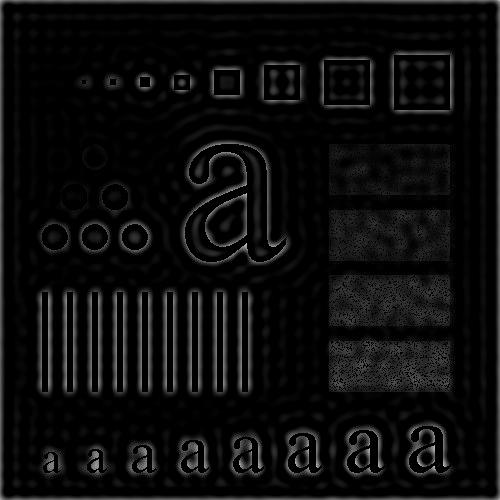
\includegraphics[width=0.33\textwidth]{../data/ideal_highpass_60_characters_test_pattern.jpg}
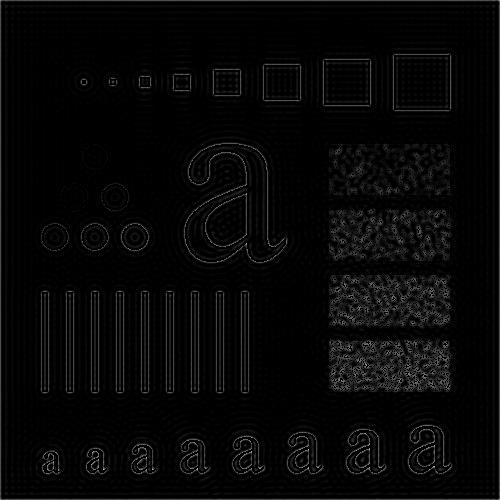
\includegraphics[width=0.33\textwidth]{../data/ideal_highpass_160_characters_test_pattern.jpg}

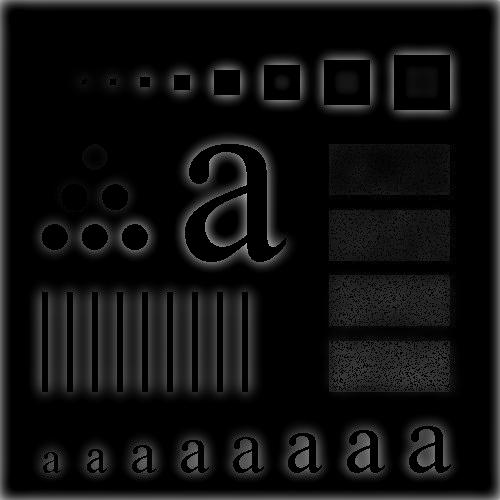
\includegraphics[width=0.33\textwidth]{../data/butterworth_highpass_30_characters_test_pattern.jpg}
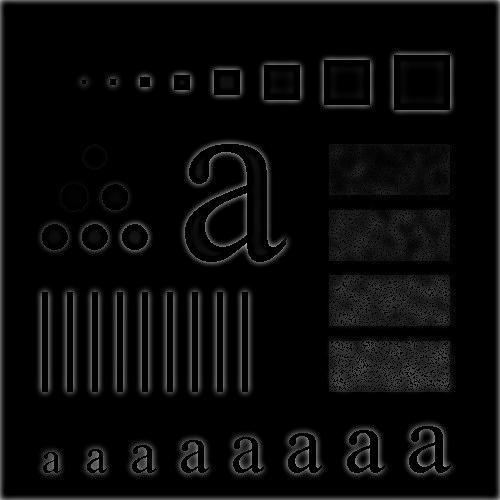
\includegraphics[width=0.33\textwidth]{../data/butterworth_highpass_60_characters_test_pattern.jpg}
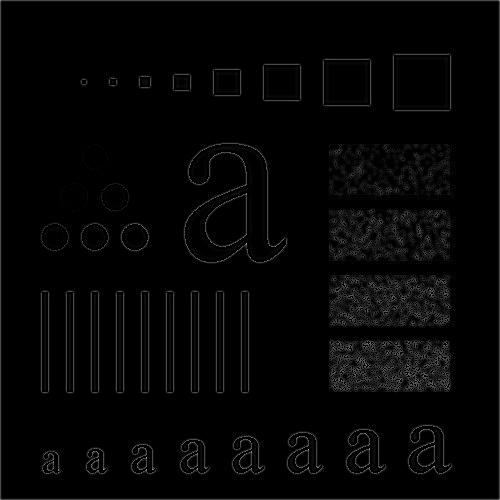
\includegraphics[width=0.33\textwidth]{../data/butterworth_highpass_160_characters_test_pattern.jpg}

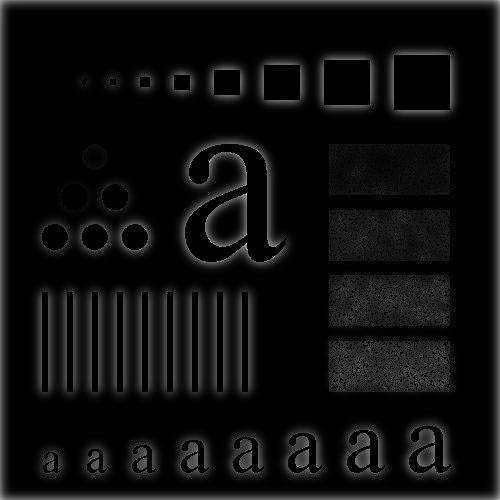
\includegraphics[width=0.33\textwidth]{../data/gaussian_highpass_30_characters_test_pattern.jpg}
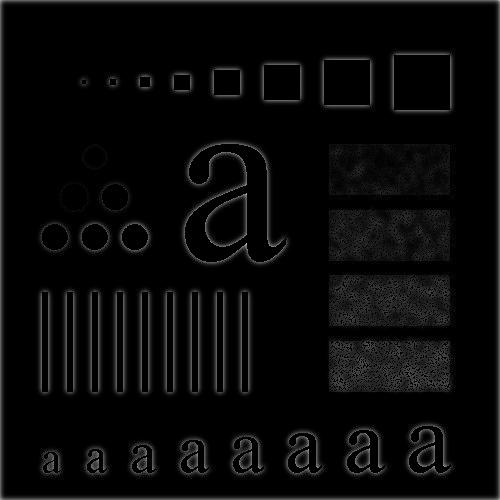
\includegraphics[width=0.33\textwidth]{../data/gaussian_highpass_60_characters_test_pattern.jpg}
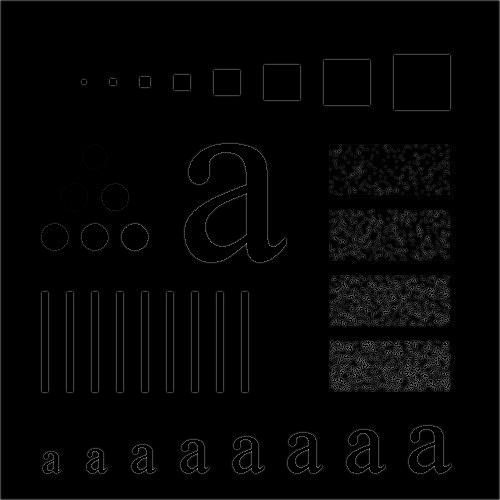
\includegraphics[width=0.33\textwidth]{../data/gaussian_highpass_160_characters_test_pattern.jpg}

\end{document}